\chapter{Разработка КИМ пространственной модели и исследование динамики управления ОЭП при действии возмущений} \label{ch:ch5}

\section{КИМ трехфазного моментного привода} \label{ch:ch5/sect1}

Используя уравнения полученые в разделе \ref{ch:ch3/sect9} составим компьютерную модель привода.
В соответствии с системой уравнений (\ref{eq:p3:9.1}) составим структурную схему привода:
\begin{figure}[ht]
	\centering
	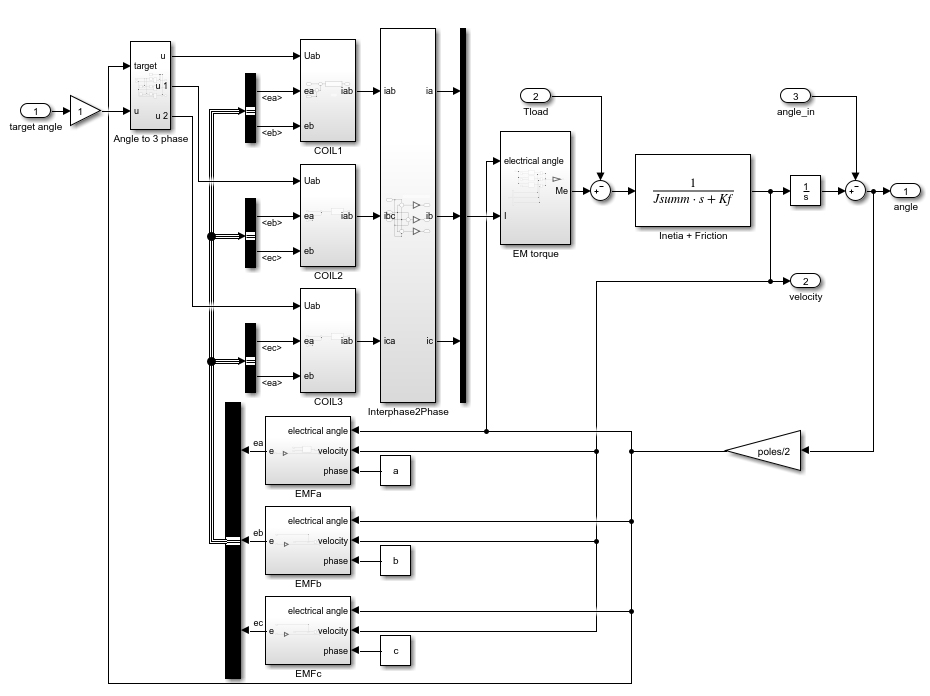
\includegraphics[width=1.0\linewidth]{motor} 
	\caption{Схема модели трехфазного ДБМ}
	\label{fig:motor}
\end{figure}

Часть уравнения учитывающая зависимость напряжения фазы от тока описывается блоком COILx, где номер фазы. Структура блока показан на рисунке \ref{fig:motor_coil}.

\begin{figure}[ht]
	\centering
	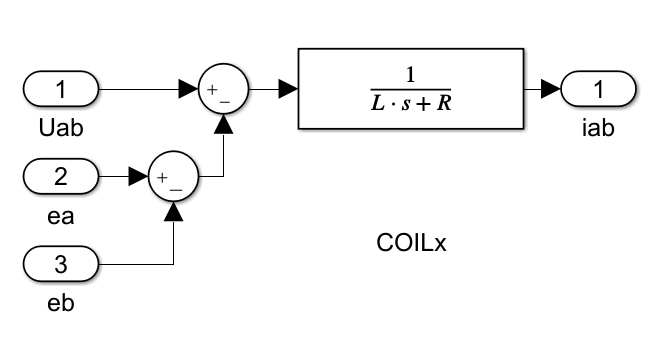
\includegraphics[width=0.4\linewidth]{coil} 
	\caption{Схема блока COILx}
	\label{fig:motor_coil}
\end{figure}

Для преобразования межфазных токов в фазовые введен блок "Interphase2Phase", его структура показана на рисунке \ref{fig:CC}.

\begin{figure}[ht]
	\centering
	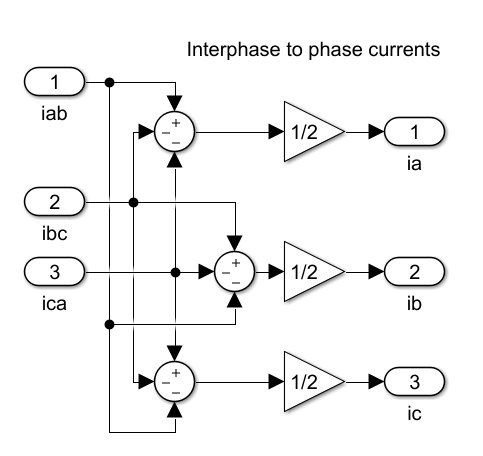
\includegraphics[width=0.3\linewidth]{CC} 
	\caption{Схема пересчета токов}
	\label{fig:CC}
\end{figure}

Уравнение (\ref{eq:p3:9.4}) реализовано в блоке моделирующем электромагнитный крутящий момент силы привода (рисунок \ref{fig:EMT}).

\begin{figure}[ht]
	\centering
	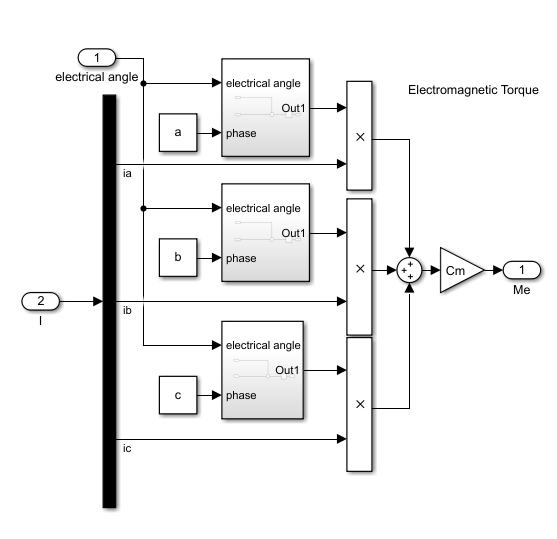
\includegraphics[width=0.5\linewidth]{EMT} 
	\caption{Блок моделирования электромагнитного крутящего момента силы привода}
	\label{fig:EMT}
\end{figure}

Пользуясь уравнением (\ref{eq:p4:s3.1}) или его нелинеаризованной формой (\ref{eq:p3:49}) можно вычислить угловую скорость для определения обратнонаведенного ЭДС, участвующую в уравнении (\ref{eq:p3:9.1}). Уравнение связывающее угловую скорость привода и обратнонаведенную ЭДС, описанное формулой (\ref {eq:p3:9.2}), моделируется блоком EMFx (рисунок \ref{fig:EMF}).

\begin{figure}[ht]
	\centering
	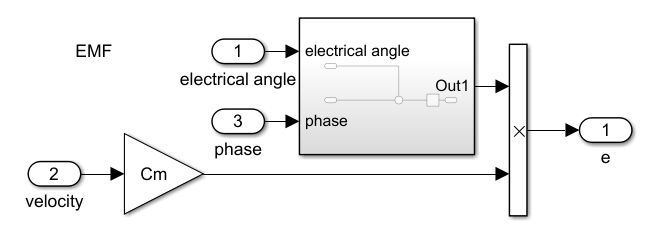
\includegraphics[width=0.5\linewidth]{EMF} 
	\caption{Блок моделирования обратнонаведенной ЭДС}
	\label{fig:EMF}
\end{figure}










Для проверки модели привода и сравнения результатов моделирования с упрощенной моделью составлена КИМ10 (рисунок \ref{fig:KIM10}). Уравнения привода дополнены блоком "Inertia + Friction" (рисунок \ref{fig:motor}) описывающем механическую составляющую модели привода.
 
\begin{figure}[ht]
 	\centering
 	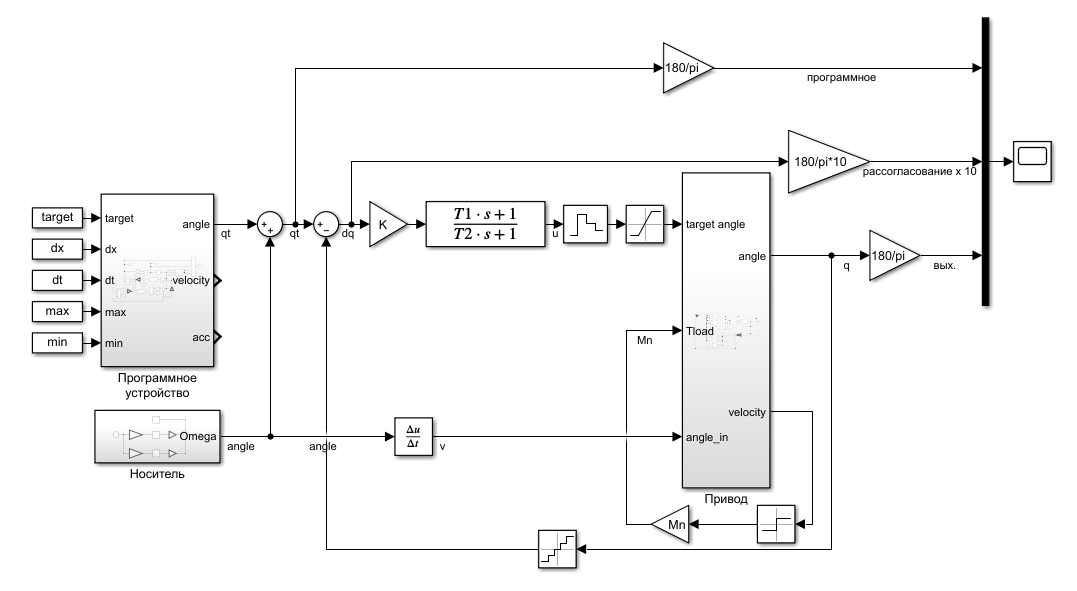
\includegraphics[width=1.0\linewidth]{system} 
 	\caption{Процессы наведения ОЭП по каналу азимута}
 	\label{fig:KIM10}
\end{figure}

Реальный привод управляется тремя сигналами, для моделирования изолированного канала системы в целом необходимо добавить блок "Angle to 3 phase" (рисунок \ref{fig:a2p}).

\begin{figure}[ht]
	\centering
	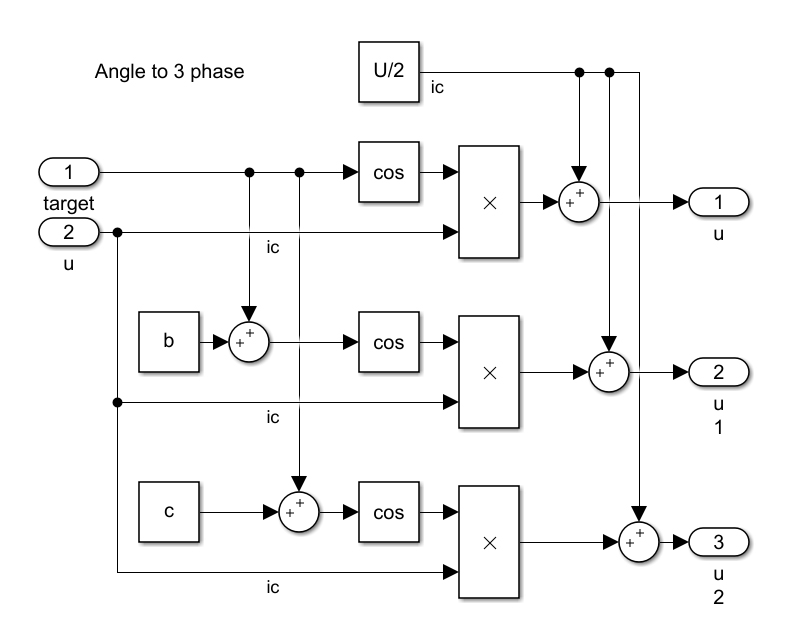
\includegraphics[width=0.6\linewidth]{A23P} 
	\caption{Блок преобразования угла в управляющие сигналы трех фаз}
	\label{fig:a2p}
\end{figure}

Построим переходные процессы для полученной модели
















\section{Компьютерная имитационная модель двухканальной САУ ОЭП  } \label{ch:ch5/sect2}

Используя  уравнения из глав \ref{ch:ch3} и \ref{ch:ch4} составим структурную схему системы управления с объектом управления.
 
\begin{figure}[ht]
	\centering
	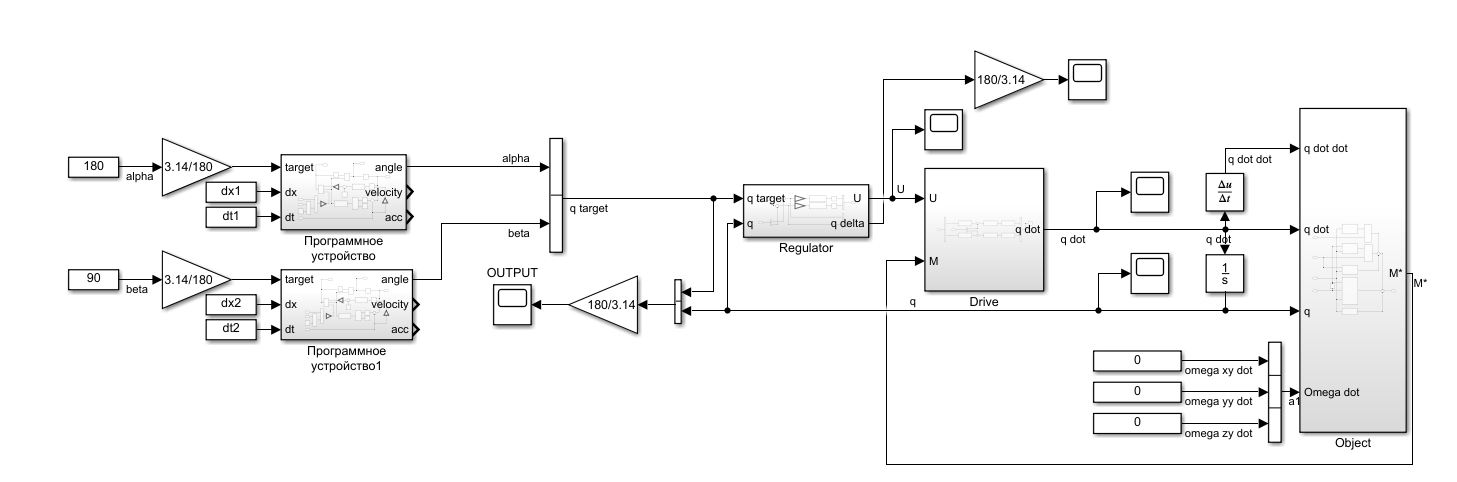
\includegraphics[width=1.0\linewidth]{C5_1} 
	\caption{Структурная схема САУ ОЭП}
	\label{fig:structure}
\end{figure}

Блоки программных устройств реализуют управляющее воздействие, состав блока описан в \ref{ch:ch4/sect2+}.
Блок "Regulator" реализует корректирующее звено в контуре управления.
В блоке "Drive" заключена модель трехфазного привода, состав блока и подробное описание обсуждалось в разделе \ref{ch:ch5/sect1}.
Блок "Object" реализует уравнения математической модели объекта управления в виде представленом в главе  \ref{ch:ch3}. Состав и подробное описание блока приводится ниже в разделе \ref{ch:ch5/sect3}.

Результат моделирования без учета движения борта представлен на рисунках \ref{fig:s5delta}


\begin{figure}[ht]%
	\centering
	\subfloat[Рассогласование системы]{{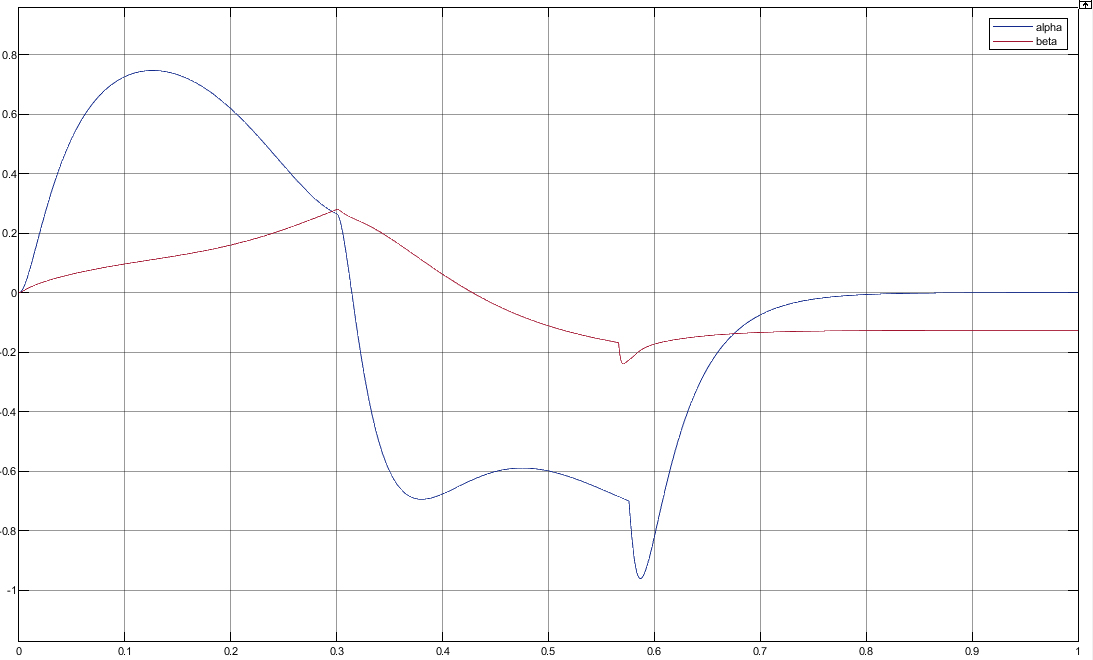
\includegraphics[width=0.45\linewidth]{c5delta} }}%
	\qquad
	\subfloat[Графики переходных процессов системы]{{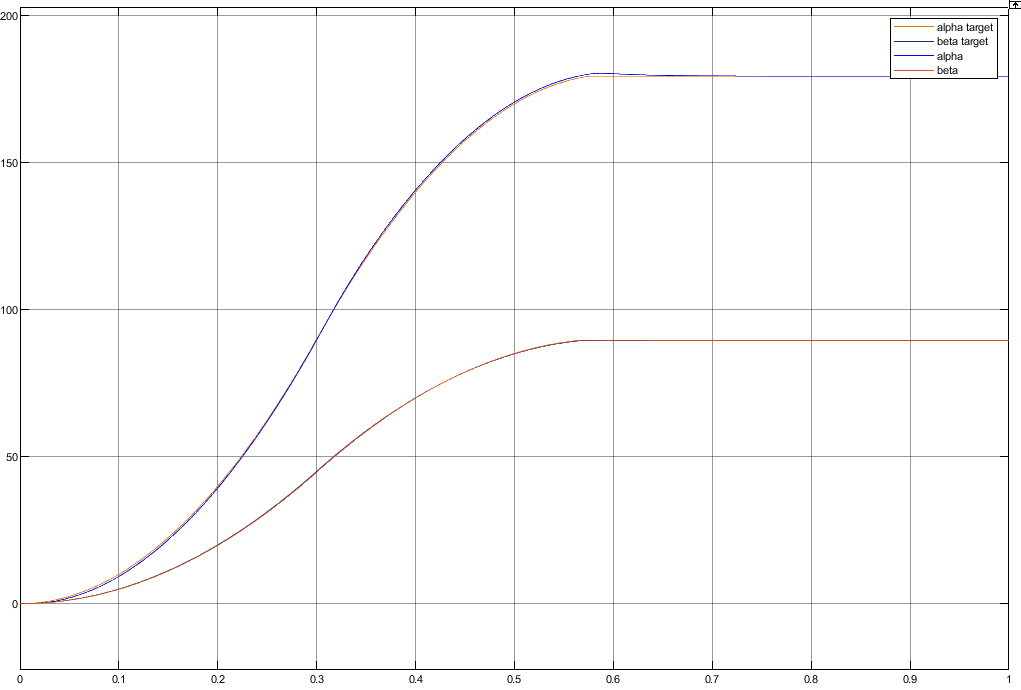
\includegraphics[width=0.45\linewidth]{c5io} }}%
	\caption{Графики переходных процессов системы по двум каналам (градусы)}%
	\label{fig:s5delta}%
\end{figure}



Рассогласование САУ по каналу азимута не превышает 1 градуса, а по углу места не превышает 0.3 градусов (рисунок \ref{fig:s5delta}). По сравнению с моделированием изолированных каналов ошибка возросла в следствии влияния перекрестных связей.



\newpage

\section{Разработка компьютерной имитационной модели ЦСАУ ОЭП с учетом  движения борта} \label{ch:ch5/sect3}


На основе синтезированных регуляторов САУ и с учетом указанных нелинейностей разработаны КИМ ЦСАУ (рисунок \ref{fig:digital_az}). Модели с учетом нелинейностей КИМ позволяют изменять величины дискретности датчика, частоту ШИМ усилителя и насыщения в УМ и проводить исследования динамики нелинейной САУ при заданных пределах этих параметров. 
\begin{figure}[ht]
	\centering
	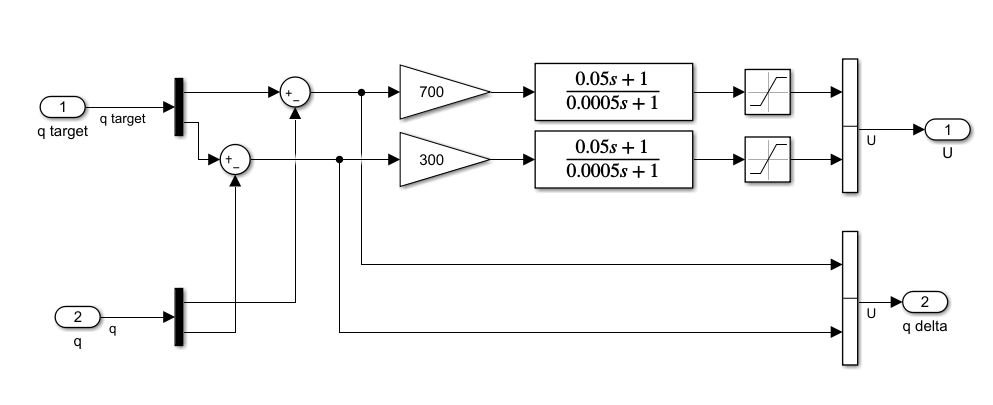
\includegraphics[width=0.8\linewidth]{C5_2} 
	\caption{Блок моделирующий корректирующее устройство системы управления}
	\label{fig:coorection}
\end{figure}

\begin{figure}[ht]
	\centering
	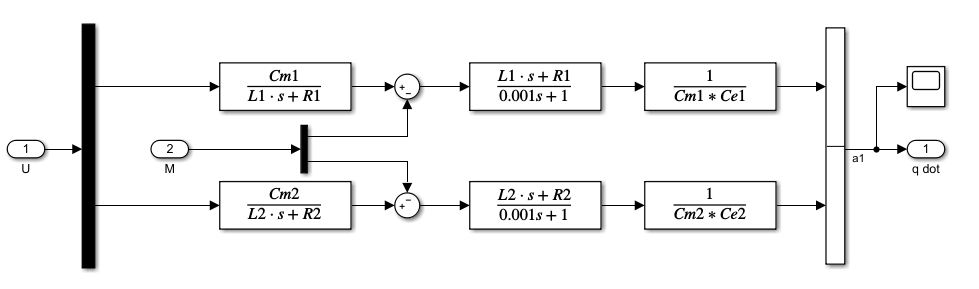
\includegraphics[width=0.8\linewidth]{C5_3} 
	\caption{Блок моделирующий объект управления (линеаризованная система)}
	\label{fig:object_lin}
\end{figure}

 Модель объекта управления описывается уравнением (\ref{eq:p3:48}). Воплащение данного уравнения в модели осуществляется блоком "Object". На рисунке \ref{fig:object} показан состав этого блока.
\begin{figure}[ht]
	\centering
	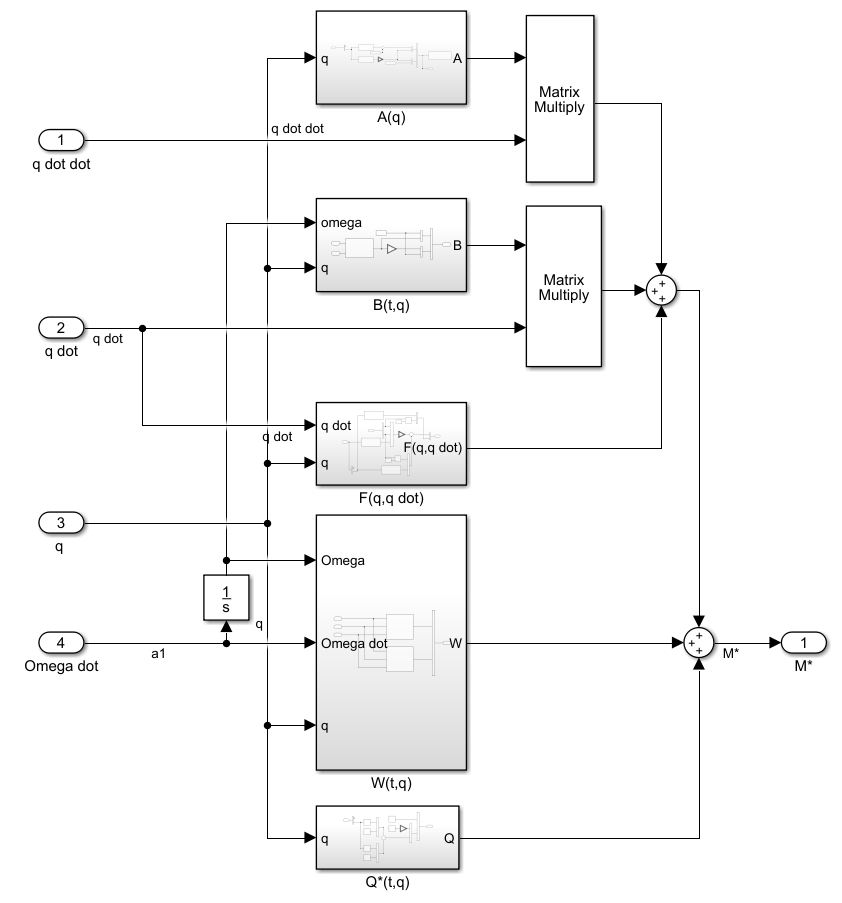
\includegraphics[width=0.8\linewidth]{C5_4} 
	\caption{Модель объекта управления в соответствии с (\ref{eq:p3:48})}
	\label{fig:object}
\end{figure}

\newpage

\section{Исследование динамики наведения и стабилизации ОЭП} \label{ch:ch5/sect4}
\begin{figure}[ht]
	\centering
	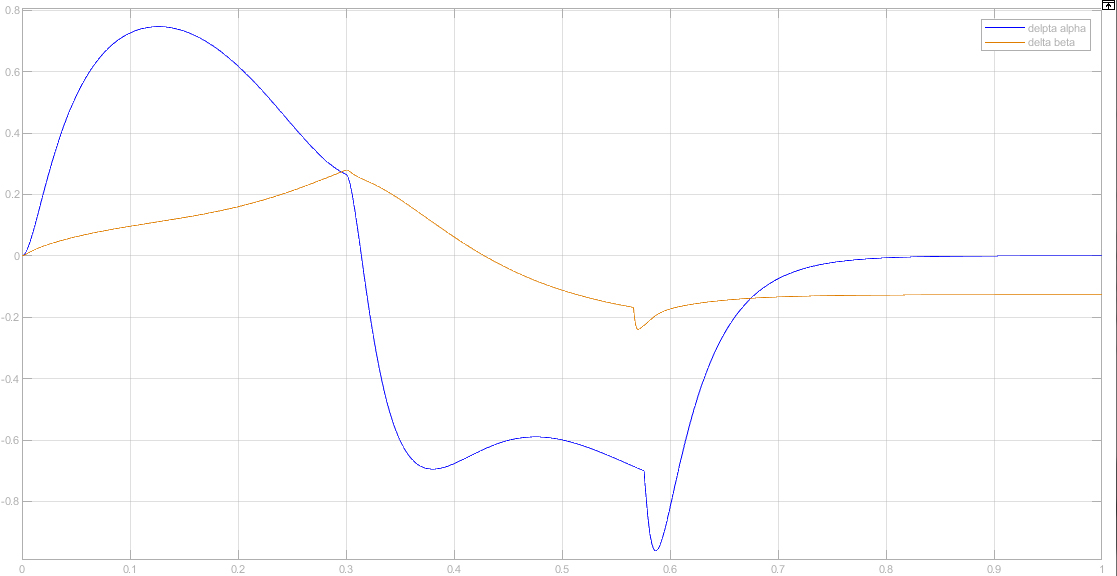
\includegraphics[width=1.0\linewidth]{C5_G1} 
	\caption{Процессы наведения ОЭП по каналу азимута}
	\label{fig:az_true}
\end{figure}
\begin{figure}[ht]
	\centering
	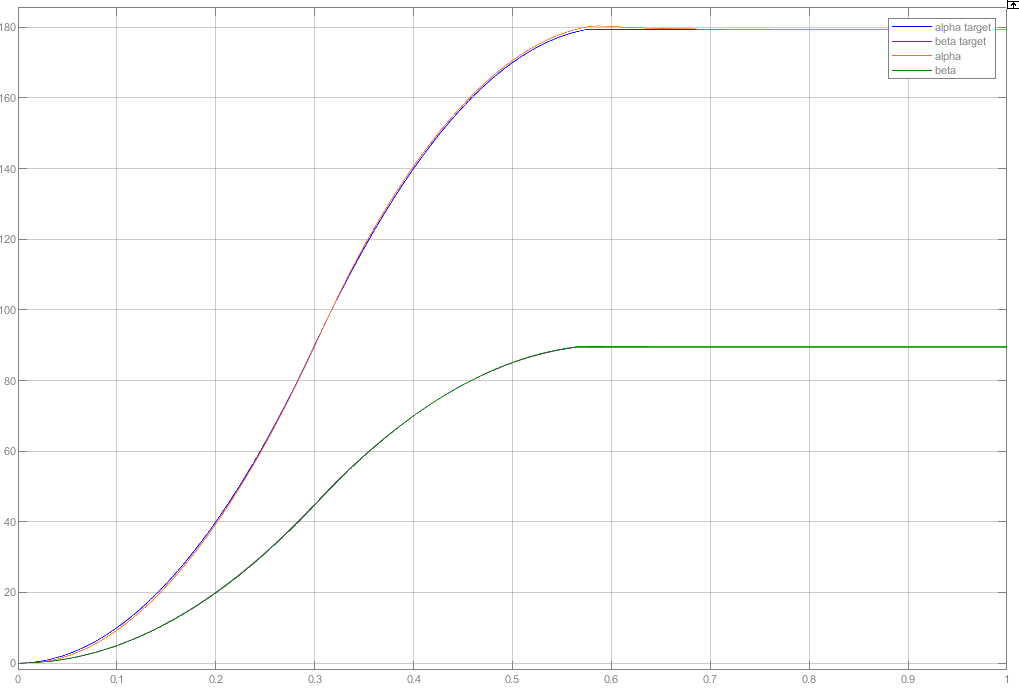
\includegraphics[width=1.0\linewidth]{C5_G2} 
	\caption{Процессы наведения ОЭП по каналу азимута}
	\label{fig:az_true}
\end{figure}
\section{Выводы} \label{ch:ch5/sect5}
	


Некоторый текст.

\clearpage